\section{Introducción}
\hspace{1mm} Se pretende diseñar amplificadores utilizando tecnologías VFA (Amplificador Realimentado por Tensión) y CFA (Amplificador Realimentado por Corriente) aplicando conceptos de compensación.

\bigskip
\hspace{1mm} Se analizarán tres circuitos amplificadores compuestos a partir de las tecnologías nombradas en el párrafo anterior. El primer circuito está conformado por dos VFA, en tanto que el segundo y tercer circuito estarán compuestos por un CFA y un VFA. El esquema de estos tres circuitos es el mismo y se presenta a continuación.

\begin{figure}[!h]
    \centering
    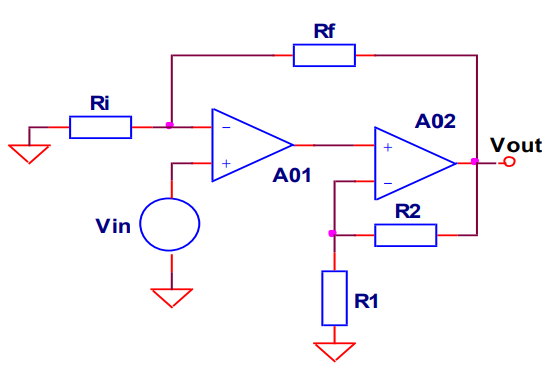
\includegraphics[scale=0.7]{img/Objetivos.png}
    \caption{Esquema del amplificador compuesto}
\end{figure}

\hspace{1mm} En el armado de los circuitos, los integrados utilizados para los VFA serán los LM324 de dos polos y, para el CFA será el LM6181 cuya transimpedancia también tiene dos polos. 

\bigskip
\hspace{1mm} Los requerimientos para dichos circuitos amplificadores son los expuestos seguidamente.
\begin{itemize}
    \item Ganancia global: \(A_{vf} = 20~dB\)
    \item Máxima planicidad de módulo: \(M_{\phi}=65°\) o \(Q_p=0.707\)
\end{itemize}


\newpage
\section{Consigna}
\subsection{Circuito I: VFA-VFA}
\hspace{1mm} Empleando la tecnología VFA y el circuito integrado LM324, proceder a realizar las siguientes consignas.
\begin{enumerate} 
    \item Diseñar el amplificador compuesto VFA+VFA.
    \item Calcular el ancho de banda potencial, la frecuencia del polo de la función de transferencia a lazo cerrado y el ancho de banda a \(-3~dB\).
     \item Medir el ancho de banda a \(-3~dB\).
     \item Estimar el margen de fase obtenido en base a la respuesta al escalón del amplificador compuesto.
\end{enumerate}


\subsection{Circuito II: VFA-CFA}
\hspace{1mm} Utilizando las tecnologías VFA y CFA, así como los circuitos integrados LM324 y LM6181, proporcionar respuesta a los siguientes apartados.

\begin{enumerate}
    \item Diseñar el amplificador compuesto VFA+CFA para máxima planicidad de módulo y que además cumpla con un ancho de banda potencial aproximado de \(f_g=2~MHz\). Tener en cuenta la presencia del segundo polo del VFA.
    \item Calcular el ancho de banda potencial, la frecuencia del polo de la función de transferencia a lazo cerrado y el ancho de banda a \(-3~dB\).
    \item Medir el ancho de banda a \(-3~dB\).
    \item Estimar el margen de fase obtenido en base a la respuesta al escalón del amplificador compuesto.
\end{enumerate}

\subsection{Circuito III: VFA-CFA}
\hspace{1mm} Insertar en la configuración anterior una red de compensación \textbf{cero-polo} (a la salida del VFA) de tal modo que el cero de la red cancele el segundo polo del VFA. Ubicar el polo de la red a una octava de su cero. Retocar la ganancia del CFA realimentado para compensar la atenuación introducida por la red. Constatar la \textbf{mejora del margen de fase} a través de la respuesta escalón. 

\hspace{1mm} Seguidamente, realizar las siguientes consignas.
\begin{enumerate}
    \item Calcular y medir el margen de fase, el ancho de banda potencial, la frecuencia del polo de la función de transferencia a lazo cerrado y el ancho de banda a \(-3~dB\).
    \item Calcular el ancho de banda potencial, la frecuencia del polo de la función de transferencia a lazo cerrado y el ancho de banda a \(-3~dB\).
    \item Medir el ancho de banda a \(-3~dB\).
    \item Estimar el margen de fase obtenido en base a la respuesta al escalón del amplificador compuesto.
\end{enumerate}

\newpage
\section{Marco teórico}

\subsection{Amplificador Realimentado por Tensión (VFA)}

\hspace{1mm} Un amplificador VFA (Voltage Feedback Amplifier, por sus siglas en inglés) es un tipo de amplificador electrónico que se utiliza para amplificar señales eléctricas, como señales de voltaje, corriente o potencia. La característica principal de un amplificador VFA es que su ganancia y comportamiento de amplificación están determinados principalmente por la retroalimentación de voltaje.

\bigskip 
\hspace{1mm} En un amplificador VFA, una parte de la señal de salida se toma y se compara con la señal de entrada original utilizando realimentación negativa. La diferencia entre estas dos señales se utiliza para generar una señal de error que se amplifica y luego se utiliza para corregir la señal de salida, manteniendo la amplificación dentro de los límites deseados y estables.

\bigskip 
\hspace{1mm} La ganancia y las características del amplificador VFA están controladas por los componentes pasivos y activos utilizados en su diseño.

\bigskip
\begin{figure}[!h]
    \centering
    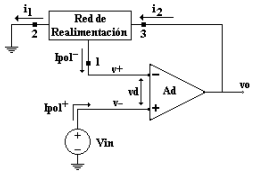
\includegraphics[scale=1]{img/VFA.png}
    \caption{VFA}
\end{figure}

\bigskip
\hspace{1mm} Este amplificador se representa interiormente por el siguiente modelo.

\bigskip
\begin{figure}[!h]
    \centering
    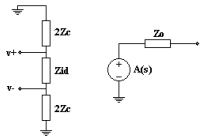
\includegraphics[scale=1]{img/VFA Modelo de amplificador real.png}
    \caption{Modelo del amplificador real}
\end{figure}

\newpage

\subsection{Amplificador Realimentado por Corriente (CFA)}

\hspace{1mm} Un amplificador CFA (Current Feedback Amplifier, por sus siglas en inglés) es otro tipo de amplificador electrónico utilizado para amplificar señales eléctricas, pero a diferencia de un amplificador VFA, su ganancia y comportamiento de amplificación están principalmente determinados por la retroalimentación de corriente en lugar de la retroalimentación de voltaje.

\bigskip
\hspace{1mm} Los amplificadores CFA tienden a tener una respuesta más rápida y una mayor banda pasante en comparación con los amplificadores VFA, lo que los hace adecuados para aplicaciones de alta velocidad, como en sistemas de comunicaciones y en ciertos equipos de medición. Sin embargo, también pueden ser más sensibles a la carga y pueden requerir un diseño más cuidadoso para mantener su estabilidad y rendimiento.

\bigskip
\begin{figure}[!h]
    \centering
    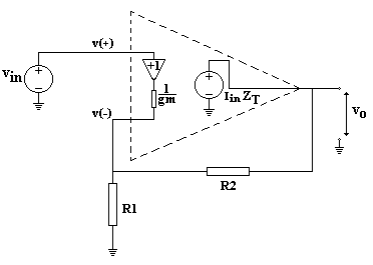
\includegraphics[scale=1]{img/CFA.png}
    \caption{CFA}
\end{figure}

\newpage
\subsection{Compensación por Adelanto}

\hspace{1mm} También denominado \textit{cero-polo} se caracteriza por generar un cero (\( f_{zx} \)) a frecuencia igual o superior al segundo polo original, corriendo de esta manera el atraso producido por este a frecuencias inferiores a la del punto crítico, mientras que el polo adjunto (\( f_{px} \)) se ubica fuera de la banda de utilización, tal que la ganancia de lazo del amplificador compensado puede expresarse como:

\bigskip
\hspace{1mm} Si \( \omega _{o2} \leq \omega _{zx} < \omega _G \) y \( \omega _{pz} \geq \geq \omega _G \)

\begin{equation}
    A_c (s) = \frac{1 + \frac{s}{\omega _{zx}}}{1 + \frac{s}{\omega _{px}}}
\end{equation}

\bigskip
\hspace{1mm} Por lo tanto.

\begin{equation}
    T'(s) = - \frac{T(0) (1 + s/\omega _{zx})}{(1 + s/ \omega _{01})(1 + s/ \omega _{o2})}
\end{equation}

\subsection{Red Paralelo Serie}

\bigskip
\hspace{1mm} Esta red esta compuesta por un capacitor y dos resistencias distribuidas de la siguiente manera.

\bigskip
\begin{figure}[!h]
    \centering
    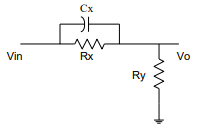
\includegraphics[scale=1]{img/Red paralelo serie.png}
    \caption{Red Paralelo Serie}
\end{figure}

\begin{equation}
    A_C (s) = \frac{V_o}{V_{in}} = \left( \frac{R}{R + R} \right) \cdot \frac{1 + sC_x R_x}{1 + sC_x (R_x // R_y)} = A(0) \cdot \frac{1 + s/\omega _{zx}}{1 + s/ \omega _{px}}
\end{equation}

\newpage
\subsection{Máxima Planicidad de Módulo}

\hspace{1mm}En aplicaciones de alta velocidad y ancho de banda, como procesamiento de señales de video y redes activas, se requieren sistemas realimentados que cumplan estrictos requisitos de ganancia, ancho de banda y distorsión de frecuencia/fase. Para optimizar el rendimiento, los amplificadores deben operar al límite de su capacidad, lo que requiere una coordinación cuidadosa entre la estabilidad del sistema y los requisitos de respuesta. Las especificaciones comunes incluyen minimizar la distorsión de frecuencia y fase en la banda de transmisión y maximizar el producto ganancia-ancho de banda. El análisis busca establecer las relaciones necesarias entre los coeficientes de la ganancia de lazo cerrado para cumplir con estos requisitos en la síntesis del sistema realimentado. Además, se considera que la ganancia del sistema en lazo cerrado presenta dos polos cuyo carácter depende de la cantidad de realimentación introducida y que la red externa al elemento activo se expresa como cociente de polinomios racionales en la variable compleja (s).

\begin{equation}
    Af(s) =  \frac{V_o}{V_{in}} = \frac{Av (s)}{1 - T(s)} = \frac{N(s)}{D(s)}
\end{equation}

\bigskip
\hspace{1mm} Dicha ecuación tiene como límites que el polinomio del denominador es como máximo de segundo grado y el polinomio del numerador no puede exceder el grado del denominador.

\hspace{1mm} Desarrollando dicha fórmula se obtiene la siguiente expresión.

\begin{equation}
    af(j \Omega) = \frac{(1 - n_2 \Omega ^2) + jn_1 \Omega}{(1 - d_2 \Omega ^2) + jd_1 \Omega}
\end{equation}

\bigskip
\hspace{1mm} Tomando módulo se deducen las relaciones que deben cumplir los coeficientes de la GLC para satisfacer la condición de máxima planicidad de módulo en la banda de transmisión.

\begin{equation}
    |af(\Omega)|^2 = \frac{(1 - n_2 \Omega ^2)^2 + (n_1 \Omega)^2}{(1 - d_2 \Omega ^2)^2 + (d_1 \Omega)^2}
\end{equation}

\begin{equation}
    |af(\Omega)|^2 = \frac{1 + a_1 \Omega ^2 + a_2 \Omega^4}{1 + b_1 \Omega ^2 + b_2 \Omega^4}
\end{equation}

\bigskip
\hspace{1mm} De la ecuación (7), función par en \( \Omega \), se infiere que la condición de invariancia del módulo con la frecuencia exige que los coeficientes de la potencias homólogas sean iguales.

\begin{equation}
    |af(\Omega)|^2 = Cte \Longrightarrow a_i = b_i \quad para \quad 0 \leq \Omega \leq \infty
\end{equation}

\bigskip
\hspace{1mm} La red que satisface esta condición se denomina pasa todo.

\bigskip
\hspace{1mm} Particularmente interesa profundizar el análisis en el caso en que N(s) sea de grado cero, por lo tanto.

\begin{equation}
    af(s) = \frac{1}{1 + \frac{s}{Q_p} + s^2}
\end{equation}

\begin{equation}
    |af(\Omega )|^2 = \frac{1}{1 + \Omega ^2 \left(\frac{1}{Q_p^2} - 2\right) + \Omega ^4}
\end{equation}

\bigskip
\hspace{1mm} Los valores de los coeficientes de esta última, en relación a la expresión general son respectivamente.

\begin{itemize}
    \item \( b_1 = \frac{1}{Q_p^2} - 2 \)
    \item \( b_2 = 1 \)
    \item \( a_1 = 0 \)
    \item \( a_2 = 0 \)
\end{itemize}

\bigskip
\hspace{1mm} De las cuales, la única que puede satisfacer para maxima planicidad de módulo.

\begin{equation}
    b_1 = a_1 \Longrightarrow Q_p = \frac{1}{\sqrt{2}}
\end{equation}

\bigskip
\hspace{1mm} Si esto se cumple, la expresión del módulo normalizado de la ganancia de lazo cerrado queda.

\begin{equation}
    |af(\Omega)| = \frac{1}{\sqrt{1 + \Omega ^4}}
\end{equation}

\bigskip
\hspace{1mm} La frecuencia de corte de \(3~dB\) deducida resulta.

\begin{equation}
    \frac{1}{\sqrt{1 + \Omega _H ^4}} = \frac{1}{\sqrt{2}} \Longrightarrow \Omega _H = 1 \Longrightarrow \omega _H = \omega _p
\end{equation}

\bigskip
\hspace{1mm} Es importante notar que en la banda de transmisión, la frecuencia normalizada \( \Omega )\) siempre es menor que uno, excepto en el extremo \( \Omega H \). Por lo tanto, el término de la potencia cuarta en la expresión del módulo tiene un impacto mínimo, lo que permite maximizar su planicidad.

\hspace{1mm} Para evaluar el margen de fase asociado a esta solución, es necesario conocer la ganancia de lazo involucrada.

\begin{equation}
    Avf (s) = \frac{Avf_i}{1 - \frac{1}{T(s)}} \Longrightarrow af(s) = \frac{1}{1 - \frac{1}{T(s)}} \approxeq \frac{1}{1 + \frac{s}{Q_p} + s^2}
\end{equation}

\bigskip
\hspace{1mm} De la cual se deduce la ganancia de lazo en términos normalizados.

\begin{equation}
    T(s) = - \frac{1}{\frac{s}{Q_p} + s^2} = - \frac{1}{s (s + \frac{1}{Q_p})}
\end{equation}

\bigskip
\hspace{1mm} La determinación de la frecuencia del punto crítico se obtiene a partir de la aplicación de la condición de módulo a la ecuación anterior con \( Q_p = 1/\sqrt{2} \)

\begin{equation}
    |T(\Omega G)| = 1 \Longrightarrow \Omega _G ^4 + \frac{1}{Q_p^2} \cdot \Omega_G^2 - 1 = 0 \Longrightarrow \Omega _G = 0,644
\end{equation}

\begin{equation}
    \omega _G = 0,644 \omega _p
\end{equation}

\bigskip
\hspace{1mm} Finalmente el margen de fase involucrado resulta.

\begin{equation}
    M \phi = \angle T(\Omega G) + 180 ^o = -90^o - tg^1 ( \Omega _G \cdot Q_p) + 180^o = 65,5^o 
\end{equation}

